\def\regenfigs{0}
\documentclass[anonymous,sigconf,9pt]{acmart}

\usepackage{microtype}
\if\regenfigs1
\usepackage{tikz,pgfplots}
\usetikzlibrary{arrows.meta}
\usepgfplotslibrary{groupplots}
\usepgfplotslibrary{external}
\usepgfplotslibrary{colorbrewer}
\pgfplotsset{cycle list/Set1}
\usepgfplotslibrary{fillbetween}
\pgfplotsset{compat=1.18}
\pgfplotsset{
    tick align=outside,
    tick pos=left,
    xmajorgrids,
    x grid style={white},
    ymajorgrids,
    y grid style={white},
    axis line style={white},
    axis background/.style={fill=white!89.803921568627459!black},
    legend style={draw=none, fill=none},
    legend cell align=left,
}
\pgfkeys{/pgf/number format/.cd, 1000 sep={\,}}

\pgfplotsset{
    log x ticks with fixed point/.style={
        xticklabel={
            \pgfkeys{/pgf/fpu=true}
            \pgfmathparse{2^\tick}%
            \pgfmathprintnumber[fixed relative, precision=4]{\pgfmathresult}
            \pgfkeys{/pgf/fpu=false}
        }
    },
    log10 x ticks with fixed point/.style={
        xticklabel={
            \pgfkeys{/pgf/fpu=true}
            \pgfmathparse{10^\tick}%
            \pgfmathprintnumber[fixed relative, precision=3]{\pgfmathresult}
            \pgfkeys{/pgf/fpu=false}
        }
    },
    log y ticks with fixed point/.style={
        yticklabel={
            \pgfkeys{/pgf/fpu=true}
            \pgfmathparse{2^\tick}%
            \pgfmathprintnumber[fixed relative, precision=4]{\pgfmathresult}
            \pgfkeys{/pgf/fpu=false}
        }
    }
}
\fi

\begin{document}

\begin{figure}[tbp]
\if\regenfigs1
\begin{tikzpicture}
\begin{axis}[
    ylabel={Speedup over CPU node},
    symbolic x coords={LJ,ReaxFF,SNAP},
    enlarge x limits=0.25,
    legend style={at={(0.45,-0.14)},
                  anchor=north,legend columns=-1},
    ybar,
    every axis plot/.append style={fill},
    ymin=-0.1,
    bar width=6pt,
    xtick=data,
    height=2in,
    width=\linewidth,
    ytick distance = 10,
]
    \pgfplotsset{cycle list/Greens-6}
    \pgfplotsset{cycle list shift=3}
    %\addplot+ table[y index=1] {results/bench.txt};
    %\addlegendentry{P100};
    \addplot+ table[y index=2] {results/bench.txt};
    \addlegendentry{V100};
    \addplot+ table[y index=3] {results/bench.txt};
    \addlegendentry{A100};
    \addplot+ table[y index=4] {results/bench.txt};
    \addlegendentry{H100};
    \pgfplotsset{cycle list/Blues-5}
    \pgfplotsset{cycle list shift=4}
    \addplot+ table[y index=8] {results/bench.txt};
    \addlegendentry{PVC};
    \pgfplotsset{cycle list/Reds-5}
    \pgfplotsset{cycle list shift=3}
    \addplot+ table[y index=5] {results/bench.txt};
    \addlegendentry{MI250X};
    \addplot+ table[y index=6] {results/bench.txt};
    \addlegendentry{MI300A};
\end{axis}
\end{tikzpicture}
\else
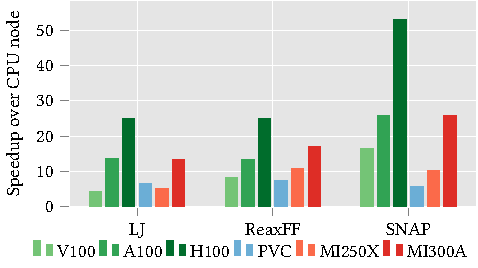
\includegraphics{generated-figures/paper-figure5.pdf}
\fi

\caption{Performance comparison of different generations of GPU hardware from NVIDIA, AMD and Intel GPUs for the three performance case studies (LJ: 16M atoms, ReaxFF: 465K atoms, SNAP: 64K atoms). The performance is normalized by the performance on a 36-core Skylake CPU node, using the base non-Kokkos LAMMPS code and MPI. Note that the Intel PVC and AMD MI250X performance was measured on one stack and GCD respectively, i.e., ``half the GPU''.}\label{fig:arch-perf}
\end{figure}

\end{document}

